

\section{Finite elements simulation}
We will now shift our focus to a more general grid which is based on triangulation. In this section we will compare our parallel implementation from the previous section and disect the differences and similarities. For that reason we shall use the same sources in our grid as given in \texttt{sources.dat}. \\
Note that the sections for the exercises will be labeled as (2.1, 2.2, 2.3, ...) corresponding to exercises (4.1, 4.2, 4.3, ...) in the lab manual.\\
\subsection{Code understanding \& \texttt{Exchange\_Borders}}
The first step is to read through the code in \textbf{MPI\_Fempois.c} and to understand it. Furthermore, we have to implement the \texttt{Exchange\_Borders} function for which only a skeleton is given. The function should exchange the border values of the local grid with the neighboring processes.\\ 
The implementation of this function is quite straight forward. We only have to loop over all the neighbors of a process and send out the border values and receive the border values from the neighbors. The function is implemented as follows:

\begin{lstlisting}[language=c]
void Exchange_Borders(double *vect)
{
    for (size_t i = 0; i < N_neighb; ++i)
    {
        MPI_Sendrecv(vect, 1, send_type[i], proc_neighb[i], 0, //send
                     vect, 1, recv_type[i], proc_neighb[i], 0, //recv
                     grid_comm, &status);
    }
}
\end{lstlisting}

\subsection{Time benchmarking}
Next we turn our attention to timing of different sections in the code. \\
We have to measure: 
\begin{itemize}
    \item Time spent in computation 
    \item Time spent exchanging information with neighbors
    \item Time spent doing global communication
    \item Idle time
\end{itemize}
We setup the following variable to measure / deduce the time spent in the different sections:
\begin{lstlisting}[language=c]
    double total_time = 0.0;
    double exchange_time_neighbors = 0.0;
    double exchange_time_global = 0.0;
    double compute_time = 0.0;
\end{lstlisting}

We will measure the time spent in computations by timing the solve function and subtracting the time spent in the \texttt{MPI\_Allreduce} calls. The time spent in the \texttt{MPI\_Allreduce} calls is the time spent in global communication. The time spent in exchanging information with neighbors is the time spent in the \texttt{Exchange\_Borders} function. Finally, the idle time can be determined by summing up the differences between the cores total time and the slowest cores total time. \underline{Note} that this way of calculating the idle time is an approximation since it is assumed that the slowest core doesn't have any idle time. However, I've discussed this with the TA and he said that this is a valid way of calculating the idle time for this exercise.\\
The commandline output for runs is as shown in \autoref{fig:timing2} for an example run: 
\begin{figure}[H]
    \centering
    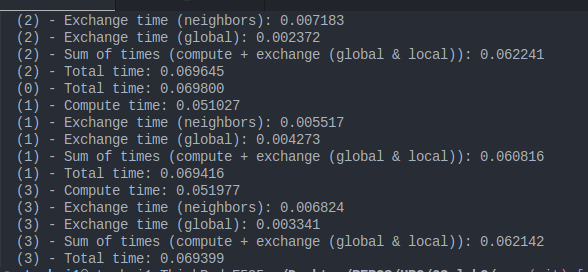
\includegraphics[width=0.7\textwidth]{../fig/lab2/ex2.png}
    \caption{Timing for the different sections.\\
    (x) \dots denotes the process rank\\
    Compute time \dots time spent in the \texttt{solve} function \underline{only on computing}\\
    Exchange time (neighbors) \dots time spent in \texttt{Exchange\_Borders} \\
    Exchange time (neighbors) \dots time spent in \texttt{MPI\_Allreduce} calls \\
    Sum of times \dots total time spent in compute and communication (excluding setup / idle time)\\
    Total time \dots total time spent in the program\\
    }
    \label{fig:timing2}
\end{figure}

The \underline{idle time} is calculated as denoted above and therefore not shown in the output in \autoref{fig:timing2}. We get the following results in \autoref{tab:timing}:


\begin{table}[H]
    \centering
    \begin{tabular}{|l|l|c|c|c|c|c|c|c|c|}
        \hline
        Top. & Grid Size & Total (avg) & Comp. (avg) & Ex. Neighb. (avg) & Ex. Global (avg) & Idle (avg) \\\hline
        1x4 & 100x100 & 57.0 & 32.5 & 5.6 & 13.3 & 0.6 \\\hline
        1x4 & 200x200 & 383.6 & 289.1 & 13.3 & 48.8 & 1.7 \\\hline
        1x4 & 400x400 & 2239.5 & 1886.9 & 22.2 & 206.1 & 11.6 \\\hline
        2x2 & 100x100 & 57.4 & 33.6 & 4.7 & 8.7 & 4.5 \\\hline
        2x2 & 200x200 & 348.3 & 266.6 & 15.5 & 35.0 & 4.0 \\\hline
        2x2 & 400x400 & 2313.2 & 1959.8 & 26.4 & 204.0 & 11.5 \\\hline
    \end{tabular}
    \caption{Rank averaged time benchmark for different grid sizes and topologies.\\ All times are in milliseconds.}
    \label{tab:timing}
\end{table}
We see that the total time is comparable between the two topologies for all grid sizes. Furthermore, the total runtime also increases non-surprisingly with the gridsize. \\
\Shining{Why does it increase faster than linearly?}\\
One could expect, that the grid with $200\times200$ elements would take 4 times as long as the grid with $100\times100$ elements. However, the runtime roughly 7 times longer. This happens because additionally to the higher number of grid points the algorithm also takes longer (more iterations) to converge. \\
\Shining{Analysis of the different times}\\
To get a better grasp on the data a stacked bar plot, as shown in \autoref{fig:timingbar}, is created. We immediately see that the bulk of the time is spent on computing the solution. The second biggest contributor is the global exchange time, followed by local exchange time and idle time (except for $2\times2$ on the $100\times100$ grid).\\
That computation takes up the biggest part of the time is of non surprise especially on the bigger grids this is to be expected. Rather surprisingly the global excahnge time comes in second. This begs the question why two lines of the form:
\begin{lstlisting}[language=c]
MPI_Allreduce(... , ... , 1, MPI_DOUBLE, MPI_SUM, grid_comm);
\end{lstlisting}
take up this much time. This actually comes down to masked idle time. While the operation itself only sums up the values of 4 double, the operation is blocking and therefore the other cores have to wait for the slowest core to finish. If we look back at the definition of idle time, we defined it as the difference of the total time of the slowest core and the total time of the current core. However, as stated above, this does not take waiting time in MPI calls (like \texttt{MPI\_Allreduce}) into account. Certainly, this explains now that the global exchange time is high, because every core has to wait for the others to synchronize to compute the \texttt{MPI\_Allreduce}.\\
\begin{figure}[H]
    \centering
    \begin{minipage}{0.48\textwidth}
        \centering
        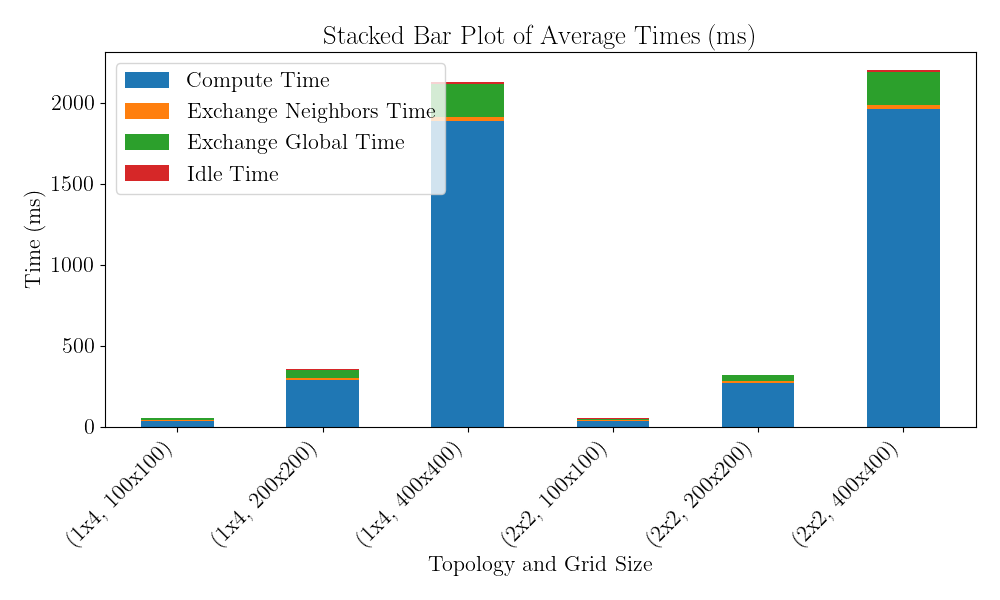
\includegraphics[width=\linewidth]{../fig/lab2/average_times_stacked_bar_22.png}
    \end{minipage}%
    \hspace{0.02\textwidth}
    \begin{minipage}{0.48\textwidth}
        \centering
        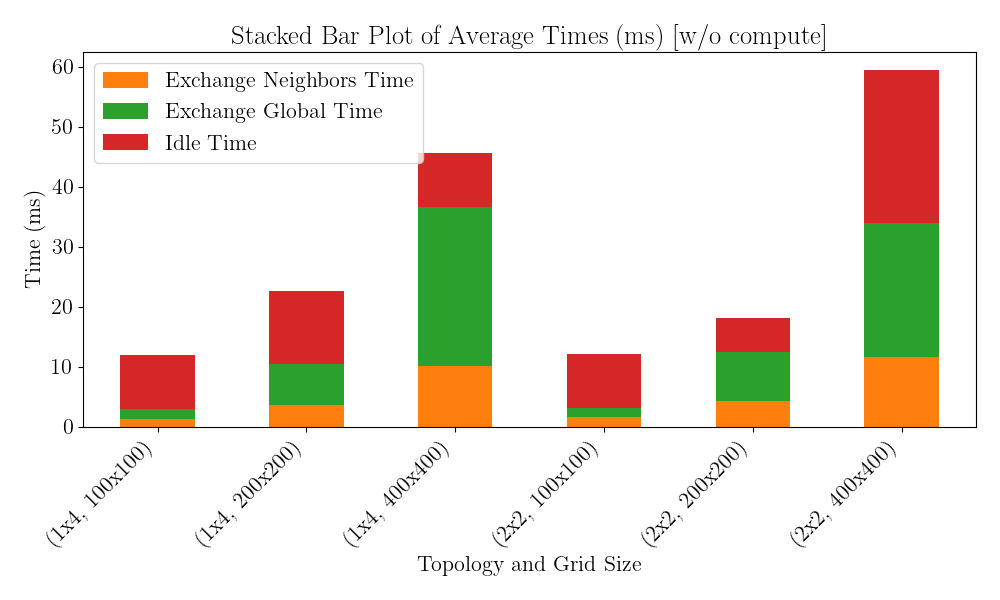
\includegraphics[width=\linewidth]{../fig/lab2/average_times_stacked_bar_no_comp_22.png}
    \end{minipage}
    \caption{Scaling behavior of the Poisson solver with different grid sizes and processor topologies}
    \label{fig:timingbar}
\end{figure}
\subsection{Data exchange amount}
This section is about the amount of data exchanged each iteration among one process with all its neighbors.\\
We assume a uniformly triangulated grid which is partitioned stripe-wise and distribution over $P$ processes. Furthermore, we assume that each process has to send the same amount of data. Indeed, this is not generally the case but for examples with periodic boundary conditions this is for example a valid assumption.\\
Now we see that every process has to communicate with $2d$ neighbors, where $d$ is the dimension of the grid, under our assumptions there are $2$ neighboring processes. With the assumption of a $n^2$ grid, our process communicates $n$ values with each of these neighbors. For striped partitioning we get: 
\begin{equation*}
    \text{Data exchanged per Process} = 2n 
\end{equation*}
or in total: 
\begin{equation*}
    \text{Data exchanged} = 2n \cdot P 
\end{equation*}
Let's check for the extreme case $1000\times1000$ grid and $P=500$ processes. We get:
\begin{equation*}
    \text{Data exchanged} = 2\cdot1000\cdot500 = 1000000
\end{equation*}
Which is the same amount of data as there are datapoints. This makes sense because every process has to communicate the top row upwards and the bottom row downwards.\\
Note, that we could even do worse if we assigned every process a single row. In this case every process would have to communicate the same data upward and downward. This would result in a data exchange of $2\cdot1000\cdot1000 = 2000000$ which is double the amount of data as there are datapoints.\\
For a box partitioning a process has to communicate $\nicefrac{n}{\sqrt{P}}$ (assuming divisibility with all neighbors) with each of its 4 neighbors. We get:
\begin{equation*}
    \text{Data exchanged per Process} = 4 \cdot \nicefrac{n}{\sqrt{P}}
\end{equation*}
or in total: 
\begin{equation*}
    \text{Data exchanged} = 4 \cdot n \cdot \sqrt{P}
\end{equation*}
This means that a striped partitioning is less efficient compared to a boxed partitioning starting from $P=4$, as can be seen in \autoref{fig:dataexchange}.\\
\begin{figure}[H]
    \centering
    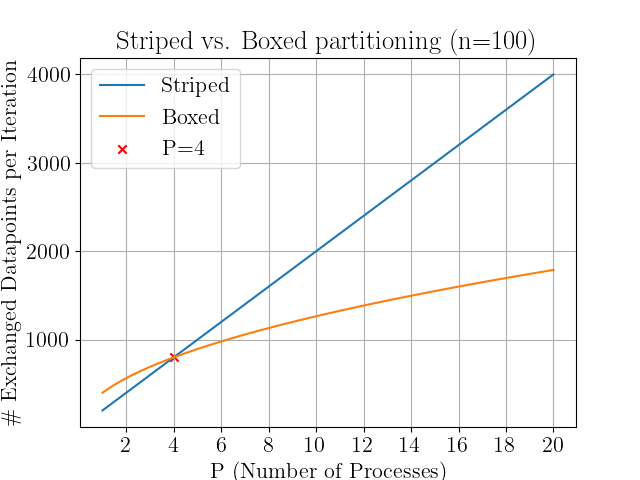
\includegraphics[width=0.5\textwidth]{../fig/lab2/scale23.png}
    \caption{Striped vs. Boxed partitioning on a $100\times100$ grid using $P$ processors.}
    \label{fig:dataexchange}
\end{figure}
\subsection{Unbalanced communication}
In the last section we assumed that every process has to communicate with the same amount of neighbors in our given scenario. That is actually not entierly true. There is an imbalance, even if just a small one.\\ 
\Shining{But where does this imbalance come from?}\\
Let's take a look at a \Shining{uniformly triangulated grid} with $P=4$ processes. We assume that the grid is box-partitioned as given in \autoref{fig:boxpart24}.\\
\begin{figure}[H]
    \centering
    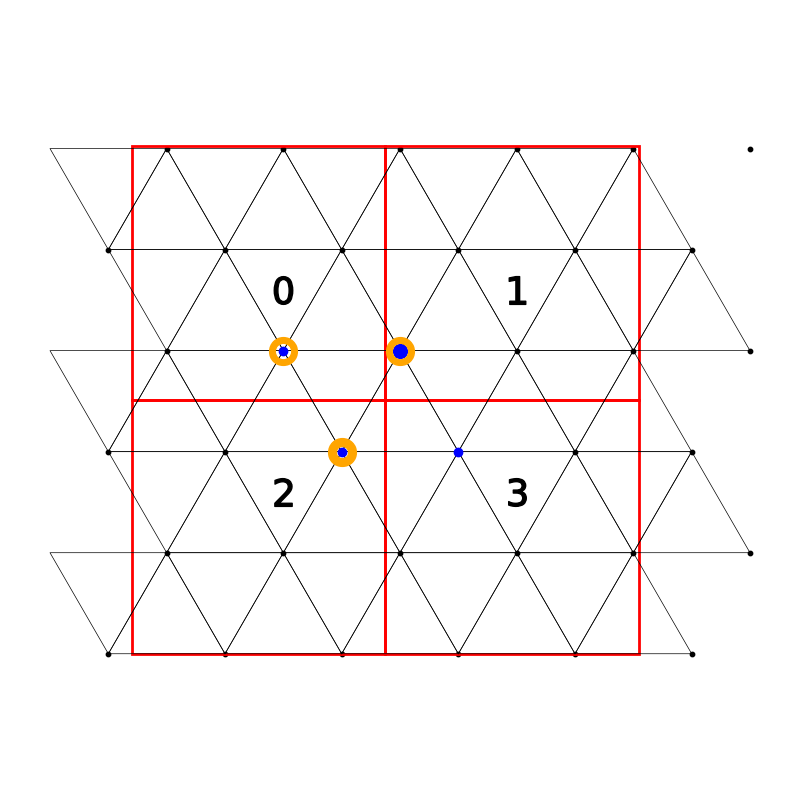
\includegraphics[width=0.5\textwidth]{../fig/lab2/grid24.png}
    \caption{Box partitioning of a uniformly triangulated grid with $P=4$ processes.\\
    One point (big-blue) in $1$ (and similarly in $3$) has to communicate its value to 3 neighbors (small-blue).\\
    Another point (big-orange circle) in $2$ (and similarly in $4$) has to communicate its value to 2 neighbors (small-orange circles).}
    \label{fig:boxpart24}
\end{figure}
We see that the geometry of a given uniform triangulated grid leads to an imbalance in communication. This imbalance is usually not a big problem, especially for bigger grids with comparably small amounts of processors because only 2 points have to communicate with 3 neighbors. However, for smaller grids or proportionally high processor counts the imbalance is more significant.\\ 

Looking at a $3\times3$ grid with $P=9$ processors, we see that the imbalance is more significant as shown in \autoref{fig:boxpart243}.\\
\begin{figure}[H]
    \centering
    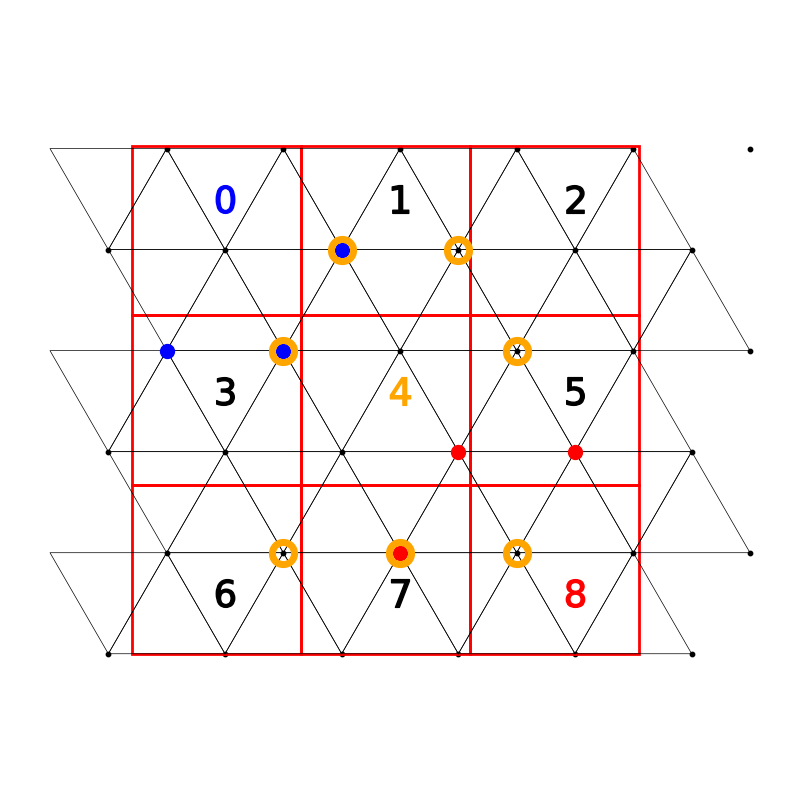
\includegraphics[width=0.5\textwidth]{../fig/lab2/grid_3x3_partition.png}
    \caption{Box partitioning of a uniformly triangulated grid with $P=9$ processes.\\
    Corner (0/8 - blue/red) processes have to communicate their values to 2 or 3 neighbors respectively (1 and 3 - blue or 4, 5 and 7 - red).\\
    Central (4 - orange) processes have to communicate their value to 6 neighbors (1, 3, 5, 6, 7 and 8).}
    \label{fig:boxpart243}
\end{figure}
As we can see the imbalance comes from the partitioning geometry on the uniform triangulated grid. Because our processor grid is rectangular the results will always, in one way or another come out as shown in the schematic above.\\
For $3\times3$ grid we have 4 corner processes which have to communicate with 2 or 3 neighbors and 1 central process which has to communicate with 6 neighbors. This is a significant imbalance and compared to the $2\times2$ grid it is not negligible, because the central process has to communicate more than 2 extra points (whole edges of datapoints) to its neighbors.\\
\subsection{Estimates for computation $\equiv$ communication time}
Let's assume that we have 4 processes and want to estimate for which grid size the computation time is equal to communication time. \\
We've already got 
\TODO{Test on DB}
\subsection{4.6}
\TODO{Run shell-script on DB}
